% Chapter 1

\chapter{Parameter tuning} % Main chapter title

\lhead{Chapter XXX. \emph{XXX}} % This is for the header on each page - perhaps a shortened title
	
%----------------------------------------------------------------------------------------

The model has several parameters which must be selected carefully before the simulation can be used to infer knowledge about market behavior. 

The parameter tuning turned out to consume a significant amount of time, and simple using a genetic algorithm to optimize over the entire space of parameters was not enough. Instead, the process was a slow and iterative one of running the genetic algorithm to create a data set, analyze the data set to find out what was discovered in the search, and then run the genetic algorithm again with different parameters. Thus several data sets were created, each with the purpose of examining some aspect of the simulation, or of the parameter tuning method itself. 

This chapter will cover the instruments used in the optimization of the model parameters, and also mention the machine learning tools used in the analysis of the data sets. 

The parameter tuning has two overall goals, which are covered in the following section.

\section{Motivation and overall procedure}
First of all, the model must be calibrated such that it mimics the behavior of real markets. Since virtually every aspect of the simulation behavior depends on the values on the various parameters, these must be chosen carefully in order for the simulation to produce realistic behavior. An example of a simulation untuned parameters causing  unrealistic behavior is given in figure \ref{subfig:unrealistic_behavior}. Selecting realistic parameters is by far a simple task. First of all, it requires a way of quantifying the quality of each simulation. The choice of such a quantification is discussed in section \ref{section:simulation_fitness}. Secondly, there might be several different parameter configurations which produce seemingly realistic behavior, but do not correspond to a realistic market setting. An example for this is given in figure \ref{subfig:unrealistic_parameters}, and section \ref{section:filtering_parameters} briefly discusses this point. 

\begin{figure}
	%issue 15
	\subcaptionbox{Parameters causing unrealistic dynamics\label{subfig:unrealistic_behavior}}
	[0.49\linewidth]{
\includegraphics[width=0.5\textwidth]{Electron.pdf}}
	\subcaptionbox{Unrealistic parameters causing realistic dynamics\label{subfig:unrealistic_parameters}}
	[0.49\linewidth]{
\includegraphics[width=0.5\textwidth]{Electron.pdf}}
	\caption{\textbf{Motivatoin for tuning:} the two}\label{fig:tuning_motivation}
\end{figure}

The second goal of the parameter tuning is to find parameters which promotes certain desirable behaviors. For instance, we might be interested in determining which parameters causes the traded price to stabilize faster after a shock to the fundamental price. Metrics for doing this is discussed in section \ref{section:simulation_fitness}

The selection of parameters is a fairly complicated process because of the large parameter space, and because it takes a significant time to evaluate the fitness of a given set of parameters\footnote{The calculation time depends largely on the parameters, such as the number of agents and how active these are. Typically one to several minutes are required to evaluate a single set of parameters.}. amount of time to execute a simulation. Because of this, the following three-step parameter selection procedure was used.
\begin{enumerate}
	\item Fix some of the model parameters in order to reduce the search space for the optimization algorithm. This requires us to consider which parameters can be fixed without losing opportunity to gain insight into market behavior. Essentially this step is a question of prioritizing the optimization of some parameters over the optimization of others. 
	\item Use an optimization algorithm to find sets of parameters which yield realistic model behavior. A genetic algorithm was chosen for this purpose, and the details are explained in section \ref{section:genetic_algorithm}.
	\item From the set of parameter combinations found by the optimization algorithm, remove the parameter combinations which obviously do not correspond to a realistic setting.
\end{enumerate}

\subsection{Selecting fixed parameters}
The main parameters of interest are the ones that control the latency and speed of the agents. The agent strategy parameters are less important, since 



\begin{description}
	%issue 16
	\item [\nrounds] Due to the computational cost of running the simulation for a large number of rounds, the the number of rounds is fixed at $10^5$ for all experiments.
	\item [Order volumes] As with most of the other agent parameters, the 
\end{description}

The remaining model parameters will either be fixed for each experiment, or varied by the genetic algorithm. 





\section{Inverse simulation with a genetic algorithm}\label{section:genetic_algorithm}
%issue 5
Inverse simulation refers to the technique of specifying metrics measuring model behavior, and then using an optimization algorithm to search for parameters resulting in desirable (or undesirable) behavior. 

In this work, a genetic algorithm was used to search the parameter space. The algorithm proceeds as explained below.
\begin{enumerate}
	\item Generate a population of healthy individuals, e.g., individuals with valid parameters.
	\item Evaluate fitness for every individual in the population.
	\item Repeat $n_\text{gen}$ times 
	\begin{enumerate}
		\item Generate offspring by crossing existing individuals.
		\item Apply mutation to with a certain probability to each individual (parents as well as children)
		\item Evaluate fitness of children and mutated parents.
	\end{enumerate}
\end{enumerate}

Mutation and crossover are the operators responsible for generating variation in the population, while the selection is responsible for propagating promising individuals to future generation where they might be improved. Several possible methods of performing each of these three steps exist in the literature (see\cite{genetic1}, \cite{genetic2}), and section \ref{section:ga_parameters} briefly covers the method and parameters of the genetic algorithm.

\subsection{Representing parameters as genes}
Since the choice of mutation and crossover operators depends on the nature of the genes, the first step towards utilizing to search the model parameters is to decide on how to encode the parameters as individuals. 
A set of parameters is represented by an individual, $i$, consisting gene for each parameter, represented by a floating point $g_{i,j}$, where $j$ denotes the index of the parameter. When the population is initialized, each $g_{i,j}$ is drawn from a uniform distributed in the range $g_j \in [0;1]$:
\begin{equation}
g_{i,j} \sim \mathcal{U}(0,1)
\end{equation}


Some of the model parameters are integers, such as \nmm and \nsc, and these are rounded after being scaled and before they are passed to the simulation.



%issue 17


\subsection{Model fitness}\label{section:simulation_fitness}

In order to use inverse simulation, it is necessary to decide on how to measure the quality of an instance of the simulation. In this work, the overall goal is to examine which parameter values cause the market to be stable, and which cause it to be unstable. 


Another interesting point is the speed with which the market responds to the shock to the fundamental price, and which parameters influence this property. Furthermore, we are interested in investigating whether or not 

\begin{itemize}
\item 'fit
\item Are there certain parameter combinations which cause the market to behave in certain ways. S
\end{itemize}
In particular the parameters controlling various time delays are of interest. 
The search space of the parameters is very large, which makes an exhaustive search impossible.
To this end, four fitness measures were defined.
The balance between the number 
Several parameters influence the number of orders submitted by the high frequency traders.

\begin{description}
\item[\roundstable < \timetoreachnewfundamental] This happens when the traded price never leaves the stability margin after reaching the new fundamental price. Note however that this case does not necessarily mean that the prices do not flicker. 
\item[\roundstable > \timetoreachnewfundamental] This happens when the traded price leaves the stability margin once or more after reaching the new fundamental. The traded price can be close to the fundamental, but flickers in and out of the stability margin as on Figure \ref{figure:tradeprice_exaples_fitness_a} shows an example where the trade price fairly stable and with no overshoot, leading to good (low) \stdev and \overshoot fitness values to be assigned to the parameters. However, even though the traded prices are mostly within the stability margin, occasional flickers out of the margin causes the simulation to score a bad (high) \roundstable fitness. Note also that \timetoreachnewfundamental is undefined in this case. 
\item[\roundstable = \timetoreachnewfundamental] This happens if a trade is executed at price $\smargin - \fas < \pmatch < \smargin + \fas$, and another trade is executed at price $\pmatch = \fas$ in the same round. 
\end{description}

\begin{figure}
\centering
\subcaptionbox{\label{figure:tradeprice_exaples_fitness_a}}
[0.49\linewidth]{\includegraphics[width=0.5\textwidth]{issue_113_tradeprice_plots/all/low_stdev_but_not_stable.png}}
\subcaptionbox{\label{figure:tradeprice_exaples_fitness_b}}
[0.49\linewidth]{\includegraphics[width=0.5\textwidth]{issue_113_tradeprice_plots/all/low_stdev_and_stable.png}}
\subcaptionbox{\label{figure:tradeprice_exaples_fitness_c}}
[0.49\linewidth]{\includegraphics[width=0.5\textwidth]{issue_113_tradeprice_plots/all/high_stdev_but_stable.png}}
\label{figure:tradeprice_exaples_fitness}
\end{figure}

\begin{description}
\item[\overshoot]
\end{description}

It is possible for a simulation to be considered stable even before

\subsection{Genetic algorithm parameters}\label{section:ga_parameters}
Although this is a basic version of genetic algorithm, using it correctly is not necessarily easy, as was encountered. First of all, the parameters for the genetic algorithm itself must be established. The larger and more complex the search space, the more resources the search will require, since the evaluating the fitness function (i.e., the running the simulation) will have to be done a larger number of times. 



Table \ref{table:genetic_algorithm_parameters} presents an overview of the parameters used in the genetic algorithm. 

\begin{table}
	\centering
	\begin{tabular}{l|l}
		Parameter & Assignment\\\hline
		Number of generations & 200 to 1000\\
		Number of individuals & 100 to 1000\\
		Cross-over points & 2\\
		Tournament size & 3\\
		Mutation probability & 0.1\\
		Mutation distribution &  $\mathcal{N}(\mu = 0, \sigma = 0.1)$\\
	\end{tabular}
	\caption{Overview of parameters used in the genetic algorithm}
	\label{table:genetic_algorithm_parameters}
\end{table}


\subsection{Controlling market behavior}
The four fitness measures defined in section \ref{section:simulation_fitness} make it possible to specify the type of market behaviour that is favoured by the genetic algorithm. gives 16 combinatinos for how to optimize the model. 

First of all, we are interested in establishing which parameters cause the market to return to a stable state after the fundamental price has incurred a shock

\begin{table}
\begin{tabular}{c|c}
\textbf{Parameter} & \textbf{Range}\\
\nmm & \\
\nsc & 
\end{tabular}
\caption{Overview of experiments}
\label{table:optimization_goals}
\end{table}


\subsection{Filtering parameters}\label{section:filtering_parameters}
As mentioned earlier, it is not enough simply to define a fitness function which assigns high values to parameters causing realistic behavior. In addition, it is important to discard parameters which obviously do not correspond to a realistic setting. Imagine that the simulation scores high fitness values when executed without any market makers. Since it is known that real markets do in fact contain market makers, nothing can be inferred from such a result. Indeed this might be a consequence of poorly designed fitness measures, but since it is easier to use domain specific knowledge to filter out the unrealistic parameters

\begin{figure}[htbp]
	\centering
		
\includegraphics{Figures/Electron.pdf}
		\rule{35em}{0.5pt}
	\caption{Example of a simulation which is assigned fairly good fitness values, but which was executed with clearly unrealistic parameters: $\nmm = \nsc = 0$. The simulation reaches the new fundamental price fairly quickly without any undershoot, and stays within the stability margin. The only point where it scores badly is the standard deviation which is slightly high due to the fluctuating trade price.}
	\label{fig:no_marketmakers}
\end{figure}


\subsection{Handling failed simulations}\label{section:failed_simulations}
\begin{figure}\subcaptionbox{\ssmmlatencymu=49, \ssmmlatencys=8, \sclatencymu=32, \sclatencys=19, \overshoot=1.0, \timetoreachnewfundamental=29210.0, \roundstable=23970.0, \stdev=0.482\label{no_reaction_0}}[0.49\linewidth]{\includegraphics[width=0.5\textwidth]{/Users/halfdan/Dropbox/Waseda/Research/MarketSimulation/Thesis/data_for_figures/test/gen0_1387987146731556L.png}}
\subcaptionbox{\ssmmlatencymu=7, \ssmmlatencys=17, \sclatencymu=21, \sclatencys=17, \overshoot=1.0, \timetoreachnewfundamental=28229.0, \roundstable=23146.0, \stdev=0.5\label{no_reaction_1}}[0.49\linewidth]{\includegraphics[width=0.5\textwidth]{/Users/halfdan/Dropbox/Waseda/Research/MarketSimulation/Thesis/data_for_figures/test/gen0_1387987146764027L.png}} \end{figure}

Some parameters cause the simulation to act in strange ways, and even crash in some cases. For instance, the the order book becomes empty, the simulation throws an exception and terminates. Similarly, if the best \bid/\ask prices drops to zero, the simulation exits. As such 

The most common odd phenomenon was the market 


\section{Applying the genetic algorithm}
Applying the genetic algorithm to produce markets with desirable behavior turned out to be more difficult that one could have hoped for. First of all, the high computational costs was a hurdle. 

Secondly, many of the data sets (see section \ref{section:gene_pool_as_data_set}) produced did not contain any useful information. 

The model parameters do influence the fitness values as they control model behavior, but they are not directly weighted into the fitness-values. This means that even after the parameters of the genetic algorithm was properly tuned in such a way that higher-fitness individuals were produced, these individuals often turned out to be of no interest. Such individuals were discarded according to the filtering criteria described in section \ref{section:filtering_parameters} would have to be discarded. An example of such a case is discussed in section \ref{}

\subsection{Time complexity}
The high time complexity stems from several factors
\begin{itemize}
\item Running a simulation for a given set of parameters required up to several minutes of computation on a single CPU core.
\item Large number of model parameters increase the size of the search space. The more parameters Unfortunately there is no magic to the way the genetic algorithm works, and optimizing in a larger search means a larger time complexity.
\item Large range of parameters. Some of the parameters are integers while some are real numbers. While most of the parameters have a lower bound, none of the parameters have upper bounds.
\item Unstable fitness parameters. Since the same set of parameters can produce varying model behavior, the fitness-values may also vary. Therefore it is necessary to evaluate the simulation several times for each set of parameters. 
\item The model parameters also influence the time complexity. For instance, evaluating a simulation with many agents takes more time than evaluating a simulation with fewer agents. 
\end{itemize}

Genetic algorithms are naturally suited for parallel computation. Two servers with a total of 40 cores and enough memory to evaluate as many simulations were utilized. With this equipment, evaluating a single strategy (see section \ref{section:datasets_introduction})for generating data sets could take 

reaching a point where the genetic algorithm began to produce useful output turned out to be somewhat of an iterative process. 


First of all, the computational cost of running the genetic algorithm was high, which meant that the algorithm was not always able to find better individuals. 

Det tager lang tid -> faerre params
skod resultater -> nye experimenter


Second of all, even when the genetic algorithm did manage to improve the fitness of the population, this did not always result in useful data. 

\subsection{Experiments: Dividing the search into parts}\label{section:datasets_introduction}
As mentioned earlier, the number of parameters and the range of each parameter influences the complexity of the search. Because of this, it is desirable to keep the number of parameters that are included in each individual as small as possible. However, fixing parameters means that some interesting properties about the model might not be discovered. Furthermore, varying all parameters at the same time makes the analysis and interpretation of the results more difficult. In an attempt to overcome this dilemma, several ``experiments'' were carried out \footnote{The reason for the quotes is that the term experiment might be stretching the common understanding of what an experiment is a little.}. Instead of trying to optimize all the model parameters at once, the search was split into several parts, each of which we call an experiment. Each of these experiments produce a data set, each of which were analyzed using the methods described in section \ref{section:data_analysis_techniques}. Some of the data sets produced interesting results, while others did not. Chapter \ref{chapter:results_and_discussion} focuses on the analysis and presents the findings. A brief overview of the experiments is presented in \ref{section:experiments_overview}, but since the motivation for creating each data set is best understood in the context of the analysis of each data set, the details are deferred until chapter \ref{results_and_discussion}. The next section will explain exactly what a data set is.

\subsection{Gene pool as data set}\label{section:gene_pool_as_data_set}
The previous sections contain the details of each of the steps undertaken in order to produce data sets. To summarize, the list below enumerates the steps.
\begin{enumerate}
\item Initialize a population in the genetic algorithm with healthy individuals.
\item Evaluate the fitness for every individual several times and obtain fitness-values by calculating averages.
\item Stack all individuals that ever lived into a $\datasetNpoints \times \individuallength$ parameter data matrix \datamatrixpar, where $\datasetNpoints$ is the number of individuals, and $\individuallength$ is the length of each individual. Likewise, stack the fitness values into a $\datasetNpoints \times \fitnesslength$ fitness-data matrix \datamatrixfit, where \fitnesslength is the number of fitness values calculated. 
\item Filter the data by removing rows in \datamatrixpar with parameters which can be deemed not to correspond to real markets, and by removing rows in \datamatrixfit with fitness values that are not realistic. Please refer to section \ref{section:filtering_parameters} for details. Naturally, when a row is removed in \datamatrixpar, it is also removed in \datamatrixfit, and vice versa. 
\item Likewise, data points which were generated by a simulation crashing before it could complete were removed.
\end{enumerate}
Tables \ref{table:example_dataset_parameters} and \ref{table:example_dataset_fitnesses} contain the first rows of \datamatrixpar and \datamatrixfit for one of the data sets.
\begin{table}
\centering
\scriptsize
\begin{tabular}{lrrrrrrrrrrrrrr}
\toprule
{} &  \sclatencymu &   \sclatencys &   \scnAgents &   \scthinkmu &   \scthinks &   \sctimehorizonmu &   \sctimehorizons &   \scwaitTimeBetweenTradingmu &   \scwaitTimeBetweenTradings &   \ssmmlatencymu &   \ssmmlatencys &   \ssmmnAgents &   \ssmmthinkmu &   \ssmmthinks \\
\midrule
0 &            84 &            11 &           14 &           98 &           9 &               1071 &               445 &                            38 &                           17 &                3 &               2 &             48 &              8 &             1 \\
1 &            23 &            21 &           74 &           49 &          24 &                529 &               554 &                            45 &                           13 &                9 &               0 &              8 &              5 &             3 \\
2 &            51 &            13 &           53 &           47 &          13 &               3586 &               536 &                            10 &                           11 &                9 &               4 &             14 &              4 &             2 \\
3 &            18 &            21 &          213 &           70 &          39 &                793 &              1179 &                            33 &                           15 &                7 &               2 &             43 &              6 &             3 \\
4 &            94 &            41 &          144 &           10 &          25 &               2668 &               893 &                            12 &                           15 &                6 &               1 &             49 &              7 &             4 \\
5 &            19 &             4 &          130 &           15 &          38 &               1085 &              1165 &                            39 &                            4 &                2 &               3 &             11 &              4 &             4 \\
6 &            65 &            15 &           91 &           81 &          46 &               3867 &              1991 &                            48 &                            1 &                7 &               2 &             21 &              4 &             4 \\
7 &            36 &            38 &          143 &           77 &          19 &               2805 &              1870 &                            10 &                            9 &                7 &               0 &              3 &              2 &             4 \\
8 &            43 &             8 &           10 &           19 &          19 &               3384 &              1706 &                            33 &                            4 &                8 &               4 &              5 &              5 &             0 \\
9 &            11 &            33 &          127 &           94 &          49 &               3597 &               723 &                            12 &                            2 &                7 &               1 &             33 &              5 &             4 \\
\bottomrule
\end{tabular}

\caption{An example data matrix containing the parameters of ten individuals who lived sometime during the execution of the genetic algorithm. In this case, each individual contained parameters for the number of HFT agents, as well as the latency and thinking time parameters. Hence, the data matrix has a column for each parameter.}
\label{table:example_dataset_parameters}
\end{table}

\begin{table}
\centering
\begin{tabular}{lrrrr}
\toprule
{} &  \overshoot &   \roundstable &    \stdev &   \timetoreachnewfundamental \\
\midrule
0 &           3 &          25359 &  0.382092 &                        29838 \\
1 &           7 &          99999 &  1.289659 &                        23373 \\
2 &           6 &          99999 &  1.253363 &                        18748 \\
3 &           7 &          99997 &  1.695150 &                        22819 \\
4 &           6 &          94343 &  1.329276 &                        22703 \\
5 &          16 &          99999 &  2.439084 &                        31860 \\
6 &           6 &          93378 &  1.287235 &                        25645 \\
7 &          10 &          99997 &  1.858166 &                        19417 \\
8 &           3 &          24039 &  0.935465 &                        27381 \\
9 &          19 &          99995 &  4.092439 &                        24845 \\
\bottomrule
\end{tabular}

\caption{This table contains the fitness values for each individual in table \ref{table:example_dataset_parameters}. Note that, in order to increase the reliability of the fitness measure of an individual, the recorded fitness-values are the average of the fitness-values obtained by evaluating each individual ten times}
\label{table:example_dataset_fitnesses}
\end{table}

\subsection{Convergence of parameters}

\section{Data analysis tools}\label{section:data_analysis_techniques}
Using inverse simulation merely creates a lot of data. This data has to be analyzed before any 

Data normalization

\subsection{Data visualization}
It is useful to be able to plot the data points 

\subsubsection{Color toned scatter plots}
Scatter plots are useful for initial data analysis, as one can quickly detect problems such as outliers, and maybe even detect clusters of data points. 

\subsection{Preprocessing}

\subsubsection{Handling outliers}
The term outliers is often used as a label for data which is considered ``invalid'' in the sense that is not a product of the true data generation process, but  due to various sources of noise. In this report, data that was caused by failing simulations corresponds to the usual understanding of outliers. However, as was already explained in section \ref{section:failed_simulations}, data from such simulations are never included in \datamatrixpar{} and \datamatrixfit{} to begin with. Instead, outliers in this report refer to entries in \datamatrixpar{} and \datamatrixfit{}  deviate significantly from the majority of the data points by having extreme values.

Such data points caused problems when applying data analysis techniques which rely on a fairly normal distribution of the data points, such as Principal Component Analysis (PCA). PCA looks for a rotation of the data space, such that the axes of the new basis are aligned with the directions of the largest variance in the original space. Since a few points with extreme values come to account for a large portion of the data set variance, the new basis computed by PCA will be aligned along these few data points. When PCA is used to extract lower dimensional features from the data set, outliers will degrade the quality of these features. In the case that PCA is used for data visualization, the scatter plots of the first few principal components will not be very informative, as they merely show the projection of the data onto the axes aligned with the outliers.

In all experiments, outliers were present in both the parameters space and in the fitness space. Outliers in the parameter space occur because of abnormally large mutations, and any dimension of the parameter space is susceptible to such an event. In the fitness space, only a few of the features suffered from the occurrence of outliers. The feature \roundstable cannot contain outliers, because the shock to the fundamental occurs at round $\round = 10^4$, and because the simulation is terminated at round $\round = 10^5$, hence $\roundstable \in [10^4,10^4+1,\hdots 10^5]$. The same is true for \timetoreachnewfundamental. \stdev and \overshoot, on the other hand, are susceptible to outliers, because the two features have no upper bound.


\begin{enumerate}
\item Apply a monotonically increasing transformation $f(x)$ to some or all of the features for every data point in the data set. A common choice of $f$ is $f(x) = \log x$, as it efficiently reduces the impact of data points with extremely high values. Figure \ref{figure:scatter_log_transform} illustrates the effect of applying the log-transform. The log-scaling does a fairly good job of reducing the importance of the outliers in the \stdev feature, while the change is less dramatic in \timetoreachnewfundamental. While the left scatter plot does not really reveal any structure of the data, the transformation makes it possible to spot to rough clusters when inspecting the right plot.

Another simple method is to manually remove 
\item Manually select one or more criteria for when a data point is to be considered an outlier. It is worth noticing that \overshoot and \stdev 
\item Use a one-class support vector machine to calculate a probability for each data point that said point is an inlier or an outlier. In this case, inliers 
\end{enumerate}

\begin{figure}\label{figure:scatter_log_transform}
\subcaptionbox{Untouched data}
[0.49\linewidth]{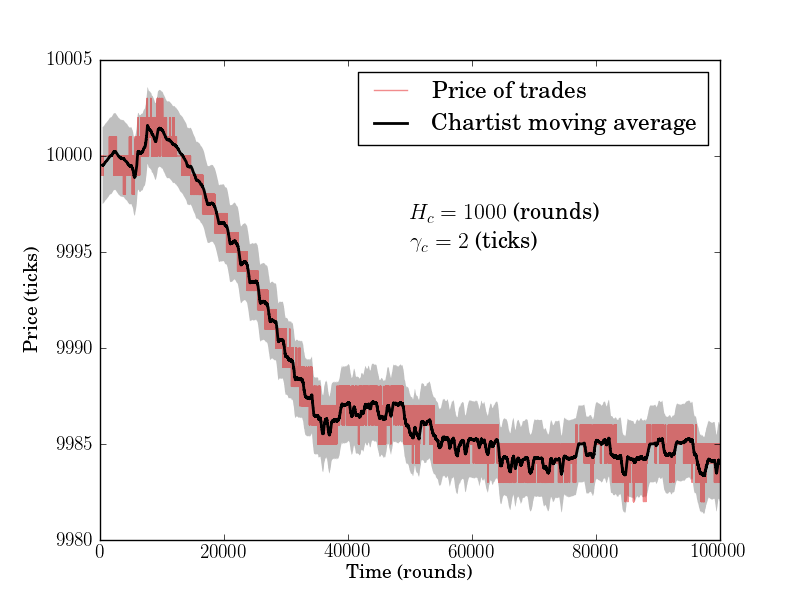
\includegraphics[width=0.5\textwidth]{21_scatter_plots/d3/f.png}}
\subcaptionbox{Log-scaled}
[0.49\linewidth]{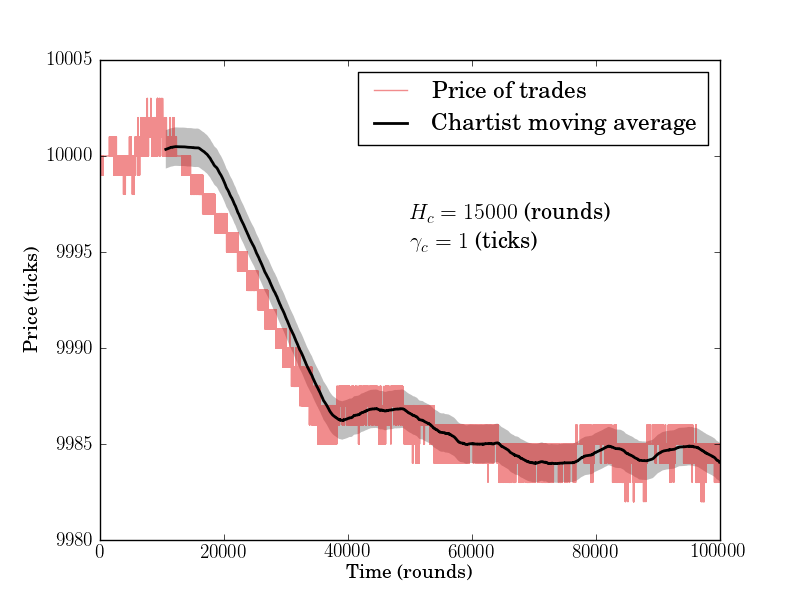
\includegraphics[width=0.5\textwidth]{21_scatter_plots/d3/g.png}}
\subcaptionbox{Outliers manually removed}
[0.49\linewidth]{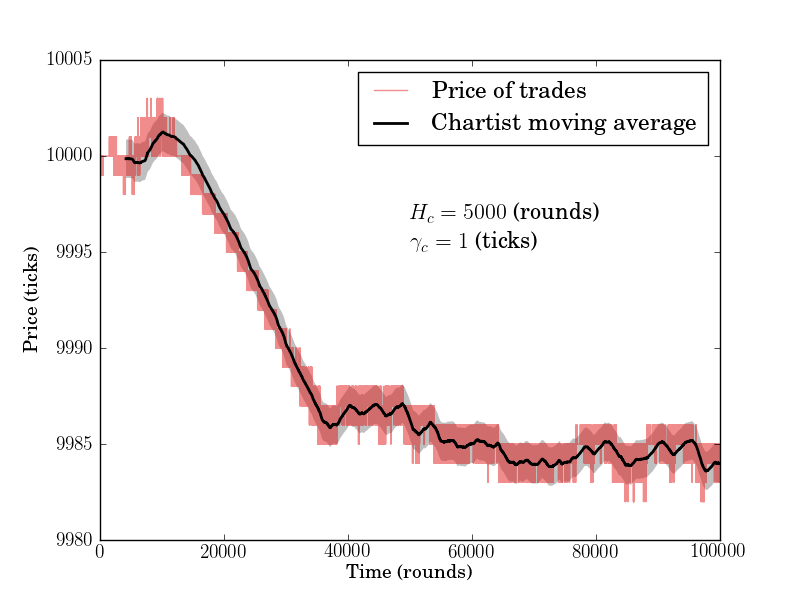
\includegraphics[width=0.5\textwidth]{103_scatter_manual_outlier/d3/a.png}}
\subcaptionbox{Log-scaled and without outliers}
[0.49\linewidth]{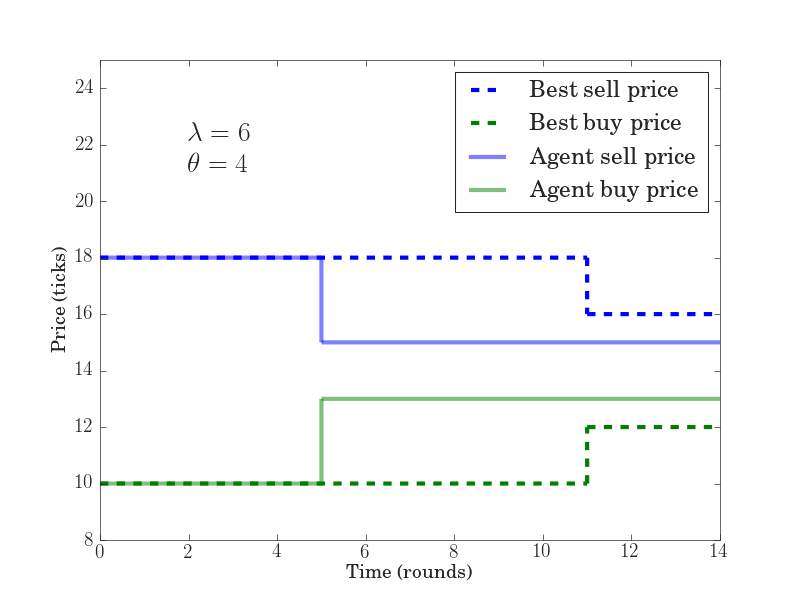
\includegraphics[width=0.5\textwidth]{103_scatter_manual_outlier/d3/b.png}}
\caption{Color toned scatter plots of \timetoreachnewfundamental, \stdev and \roundstable taken from dataset \dthree after applying log-scaling and manually removing outliers}
\end{figure}


In the parameters data set, outliers can occur due to abnormally large mutations. 
Some parameters cause the simulation to act in strange ways, and even crash in some cases. For instance, the the order book becomes empty, the simulation throws an exception and terminates. Similarly, if the best \bid/\ask prices drops to zero, the simulation exits. As such 

The most common odd phenomenon was the market 




\subsection{Clustering algorithms}
\subsubsection{GMM}
covariance type:full
